% PBilby
\chapter[Parallel Bilby]{Parallel Bilby}
\label{ch.pbilby}

\textbf{Preamble}

This chapter was originally published as:

\begin{quote}
\bibentry{pbilby}.
\end{quote}

This chapter describes \textsc{Parallel Bilby}, or \textsc{pBilby}, a parallelised implementation of \textsc{Bilby} \cite{bilby, pbilby}. 
\textsc{pBilby} uses the Message Passing Interface \cite{mpi} to distribute samplers from \textsc{dynesty} (a nested sampling package, \cite{dynesty}) over $n$-compute cores for analysis of compact-binary coalescence gravitational wave data.

Although I was not the primary author of this paper, I have played a major role in the development and maintenance of the software package \textsc{Parallal Bilby} described in this manuscript. 

% What science has been done with this

% What have i done since the publication of the paper

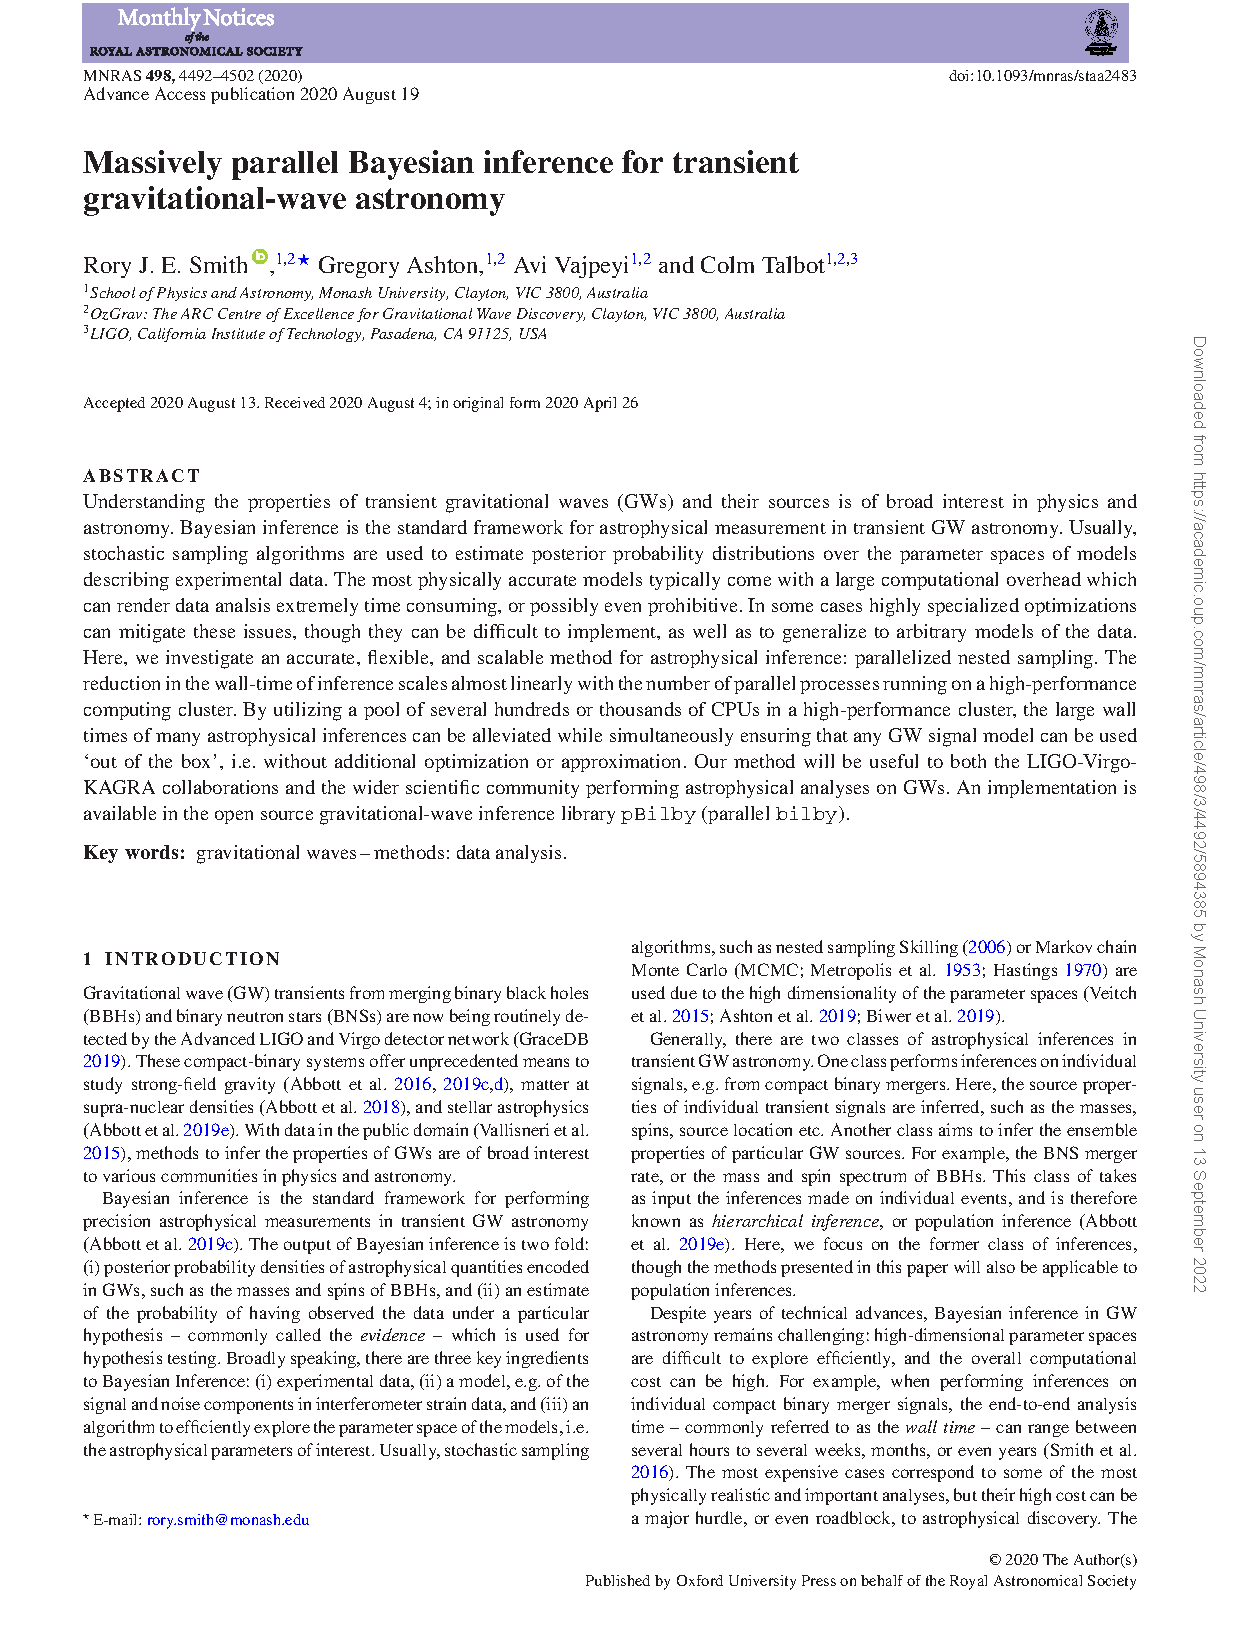
\includepdf[pages=-,pagecommand={},scale=0.93,offset=70 -80]{papers/pbilby.pdf}
